\chapter{Auswertung von Messungen: Messunsicherheit} \label{v:fehler}

%**********************************************************************************************************************
%**********************************************************************************************************************
\section{Allgemeines}

Der folgende Abschnitt zu Messungen und Messunsicherheiten ist sehr wichtig nicht nur in der Physik, sondern in allen Fächern, in denen quantitative Messungen ausgewertet und sinnvoll interpretiert werden sollen. Zunächst wollen wir verdeutlichen, was unter einer Messung überhaupt zu verstehen ist. So trivial das klingt, so hilft dieses formalisierte Verständnis doch später dabei, Begriffe wie \textit{wahrer Wert, Bestwert, usw.} zu verstehen. Im Anschluss daran werden wir uns mit der Messunsicherheit und deren Behandlung beschäftigen.

%Im Folgenden werden wir versuchen, den irreführenden Begriff des Messfehlers zu umgehen, da die Unsicherheit eines Messwertes nichts mit Fehlern während der Messung zu tun hat. Die Begriffe werden später noch genauer erklärt.

%**********************************************************************************************************************
%**********************************************************************************************************************
\section{Messung}

Die Messung einer physikalischen Größe bedeutet, diese Größe mit einer \textit{Einheit dieser Größe} zu vergleichen. Bei einer Längenmessung mit Lineal etwa, ist dessen kleinste Untereinteilung, z. Bsp. ein Millimeter, die Einheit der gemessenen Länge. Das Messergebnis ist also eine Länge in Millimetern.

Wiederholt man die Messung unter den gleichen Bedingungen, so weichen die Messwerte \textbf{immer} voneinander, und damit auch vom \textit{wahren Wert $\mu$} der Messgröße, ab. Das liegt daran, dass eine Messung niemals beliebig genau sein kann. Es hat also nichts mit einem Fehlverhalten oder einer falschen Messung zu tun, dass ein Ergebnis vom wahren Wert abweicht. Deshalb werden wir im Folgenden versuchen, den historisch benutzten Begriff des \textit{Messfehlers} zu vermeiden und stattdessen den Begriff der \textit{Unsicherheit} zu benutzen. Beide Begriffe sind in DIN 1319 wohldefiniert, und gesetzlich nicht synonym.

Die Aufgabe ist es also, aus den Messwerten den bestmöglichen Schätzwert für den wahren Wert der Größe, den \textit{Bestwert}, sowie ein Maß für dessen \textit{Unsicherheit}, zu bestimmen. 

Da es unmöglich ist, die Unsicherheit auf Null zu reduzieren, ist die Angabe eines Schätzwertes ohne seine Unsicherheit wissenschaftlich unsinnig. Die Unsicherheit einer Größe $x$ wird durch ein vorangestelltes $\Delta$ gekennzeichnet, hier also $\Delta x$. Die Angabe des Ergebnisses geschieht also in der Form
\begin{equation}
	\left( x\pm\Delta x\right)\;\mathrm{Einheit}
\end{equation}

Diese Angabe ist gleichbedeutend mit der Aussage, dass der wahre Wert der Größe der gemessenen Größe mit einer genau bekannten Wahrscheinlichkeit im Intervall $\left[x-\Delta x, x + \Delta x\right]$ liegt. Dabei ist der \textit{Fehlerintervall} als homogen zu betrachten, d.h. keiner der Werte innerhalb des Intervalls ist gegenüber den anderen Werten ausgezeichnet (keiner ist ''richtiger'' als andere) und der Zentralwert $x$ als ''Ergebniswert'' im engeren Sinne ist nicht besser oder gewichtiger als die Grenzwerte $x+\Delta x$ oder $x-\Delta x$.

%**********************************************************************************************************************
%**********************************************************************************************************************
\section{Messunsicherheiten}

Die meisten Unsicherheiten mit denen wir es im Praktikum, oder mit denen es Naturwissenschaftler in Forschung und Anwendung, zu tun bekommen, beruhen auf Unvollkommenheiten unserer Messgeräte, sowie unserem Umgang mit ihnen. Jedes Messgerät hat eine (bauartbedingte) Genauigkeit, welche die Messung begrenzt. So kann man mit einem Lineal mit Millimetereinteilung nicht sinnvoll Längen messen, die wesentlich kleiner als ein Millimeter sind.

Neben der Genauigkeit der Messgeräte spielt aber auch deren Einfluss auf die Messgröße selbst eine Rolle. Im Versuch ''Nicht stationäre Diffusion'' messen Sie zum Beispiel wie Tinte in Wasser diffundiert anhand der Lichtdurchlässigkeit der Mischung der beiden Flüssigkeiten. Da, wo Tinte hin diffundiert ist, lässt die Mischung weniger Licht durch. Die Messung geschieht, indem Sie mit einer Lampe auf die Flüssigkeit scheinen und die Helligkeit auf der anderen Seite messen. Wenn Sie die Flüssigkeit mit Licht bescheinen, erwärmt sich diese allerdings, was direkt die Diffusion beeinflusst und damit zu einem (wenn auch nur leicht) verfälschten Ergebnis führt.\\


Bei der Behandlung der Messunsicherheit ist es zweckmäßig, zwischen zwei Typen von Unsicherheiten\footnote{Auch wenn die hier gemachte Zuordnung statistische = unkorrelierte Unsicherheit, und systematische = korrelierte Unsicherheit in dieser Einfachheit sicher nicht ganz korrekt ist, ist sie für die Anwendung im Praktikum ausreichend. Vom mathematischen Gesichtspunkt ist die Korrelation zwischen den Größen und Unsicherheiten ausschlaggebend.} zu unterscheiden:
%**********************************************************************************************************************
\subsection{Systematische Unsicherheiten}

Systematische Unsicherheiten entstehen aus Effekten des Messvorgangs selbst und sind daher korreliert. Für unsere Zwecke bedeutet das, dass der Effekt für alle Einzelmessungen derselbe ist. Daraus wird klar, dass, wenn man den Effekt sehr genau kennt, es möglich ist, ihn zu korrigieren.\\
Da der Effekt über alle Messwerte korreliert ist, verringert er sich nicht, wenn man die Messung wiederholt.

Ursachen systematischer Unsicherheiten sind zum Beispiel der Einfluss des Messgerätes auf die Messgröße und falsche Eichung oder Kalibrierung des Messgeräts.\\

Beispiel: \textit{Das zur Längenmessung benutzte ''Metermaß'' ist tatsächlich nur 999~mm lang.}\\

Die Beurteilung systematischer Abweichungen, die das Messergebnis meist einseitig ver-fälschen, erfordert eine kritische Analyse aller relevanten Umstände. Es ist eine wichtige Aufgabe des Experimentators, die systematischen Abweichungen zu erkennen und zu minimieren. Da man diese nie ganz ausschalten kann, gehört eine möglichst genaue Abschätzung der verbleibenden systematischen Unsicherheit zum jedem Experiment dazu.

Allgemein gültige Regeln können dabei leider nicht gemacht werden, da die systematischen Effekte für jeden Aufbau unterschiedlich sind. Deren Abschätzung erfordert also eine kritische Auseinandersetzung mit dem jeweiligen Aufbau.
%**********************************************************************************************************************
\subsection{Statistische Unsicherheiten}

\label{ssect:StatistUnsicher}
Statistische Unsicherheiten entstehen dadurch, dass die einzelnen Messwerte bei wiederholter Messung niemals genau miteinander übereinstimmen. Gründe hierfür sind zum einen die nur endlich genaue Auflösung des Messgerätes (z. Bsp. Millimetereinteilung eines Maßbandes) und zum anderen unkontrollierbare zufällige Änderungen der Messgröße selbst (''Rauschen''). Die Abweichungen sind zwischen verschiedenen Messungen nicht korreliert, das bedeutet das Abweichungen verschiedene Beträge und Richtungen haben. Im Mittel finden ebenso viele Abweichungen um $+\Delta x$ statt, wie um $-\Delta x$. Daher können statistische Unsicherheiten durch wiederholte Messung unter gleichen Bedingungen unterdrückt werden, wenn man den Mittelwert all dieser Messungen betrachtet.

%**********************************************************************************************************************
%**********************************************************************************************************************
\section{Direkte Messung}

Eine direkte Messung liegt vor, wenn die gesuchte Größe nicht aus mehreren Messgrößen zusammengesetzt ist. Ein Beispiel wäre die Messung der Länge eines Stocks.

Direkte Messungen können prinzipiell unendlich oft wiederholt werden. Die Gesamtheit aller (unendlich vieler) Messwerte nennt man in der Statistik dann die \textit{Grundgesamtheit}. Praktisch wiederholt man eine Messung natürlich nur endlich oft, z. Bsp. $n$ mal. Die Messwerte $l_i (i=1...n)$ ergeben dann eine Untermenge der Grundgesamtheit, man nennt das eine \textit{Stichprobe}. 

Eine gängige Darstellung solcher Messwerte ist das \textit{Histogramm}, bei dem auf der x-Achse die Messwerte aufgetragen sind, auf der y-Achse die Häufigkeit, mit der der Messwert in der Stichprobe vorkommt.


%**********************************************************************************************************************
\subsection{Der Mittelwert}

Der Mittelwert, um den die Messwerte verteilt sind, nähert sich mit wachsender Anzahl $n$ von Messungen dem wahren Wert $\mu$, ist also ein guter Schätzwert für den wahren Wert basierend auf der Stichprobe der Messungen. Wenn keine besonderen Umstände vorliegen, die eine spezielle Gewichtung der Abweichung notwendig machen, verwendet man als Schätzwert das \textit{arithmetische Mittel}\footnote{Das Symbol $\sum_{i=1}^n$ bezeichnet die Summe über die Größen $x_i$, wobei die Werte aufsummiert werden, deren Zählindex $i$ zwischen 1 und $n$ liegt.}:
\begin{important}
	\begin{equation}
		\bar{x} = \frac{1}{n}\sum^n_{i=1} x_i = \frac{\left(x_1 + x_2 + ... + x_n\right)}{n} 
	\end{equation}
\end{important}

Als Messergebnis gibt man also den so definierten Mittelwert $\bar{x}$ an.

%**********************************************************************************************************************
\subsection{Die Standardabweichung}

Das arithmetische Mittel $\bar{x}$ hat die Eigenschaft, dass die Summe der Abweichungen $\Delta x_i = \left( x_i - \bar{x}\right)$ der Einzelmessungen gerade verschwindet
\begin{equation}
	\sum^n_{i=1} \Delta x_i = \sum^n_{i=1} \left(x_i - \bar{x}\right) = 0
\end{equation}
Dies folgt daraus, dass, wie in Abschnitt \ref{ssect:StatistUnsicher} erwähnt, für ein große Anzahl $n$ an Messungen, die statistischen Schwankungen symmetrisch um den Mittelwert erfolgen. Die Summe der Quadrate der Abweichungen verschwindet hingegen nicht.

Als Maß für die Breite der Streuung der Messwerte um den Mittelwert definiert man (für die Stichprobe) die \textit{Standardabweichung} $\sigma$:
\begin{important}
	\begin{equation}
		\sigma_x = \sqrt{\frac{1}{n-1}\sum^n_{i=1}\left(x_i - \bar{x}\right)^2}
	\end{equation}
\end{important}

$\sigma_x$ ist eine positive Größe, die genau dann verschwände, wenn alle Messwerte übereinstimmten, was allerdings nie passiert. 

$\sigma_x$ liefert eine Schätzung der Abweichung der Messwerte vom wahren Wert $\mu$, der allerdings unbekannt ist. Daher wird zur Berechnung von $\sigma_x$ der Mittelwert $\bar{x}$ benutzt. Für eine Einzelmessung ist diese Schätzung nicht durchführbar, was durch den Faktor $1/n-1$ berücksichtigt wird. Für $n=1$ ist $\sigma_x$ also mathematisch nicht definiert.

\paragraph{Bemerkung:}

Die Formel für die Standardabweichung kann so umgestellt werden, dass der Mittelwert zur Berechnung nicht benötigt wird. Dies ist insbesondere dann von Vorteil, wenn die Unsicherheit schon während der Messwertaufnahme berechnet werden soll, der Mittelwert also noch gar nicht bekannt ist. Zu diesem Zweck kann folgende Formel verwendet werden
\begin{equation*}
\sigma_x = \sqrt{\frac{1}{n(n-1)}\left[n\sum_{i=1}^n{x_i^2} - \left(\sum_{i=1}^n{x_i} \right)^2\right]}
\end{equation*}

%**********************************************************************************************************************
\subsection{Die Normalverteilung}

Die Standardabweichung gibt ein Maß für die mittlere Abweichung der Messwerte vom wahren Wert an. Natürlich gibt es Messwerte, die weniger abweichen und solche die mehr abweichen. Für eine sehr große Anzahl an Messwerten, $n\rightarrow \infty$, kommt jeder einzelne Messwert mit der Häufigkeit $h$ vor. Diese nennt man die \textit{Wahrscheinlichkeitsdichte}. \\
Aufgrund des \textit{zentralen Grenzwertsatzes} wird in den meisten Fällen die Häufigkeit durch die \textit{Gaußsche Normalverteilung} beschrieben:
\begin{important}
	\begin{equation}
		h(x) = \frac{1}{\sqrt{2\pi}\sigma}\cdot e^{-\frac{\left(x-\bar{x}\right)^2}{2\sigma^2}}
	\end{equation}
\end{important}

Die Gauß-Funktion (''Glockenkurve'')  ist symmetrisch um den Mittelwert $\bar{x}$ und so normiert, dass das Integral von $-\infty$ bis $\infty$ gerade 1 ergibt. 

Tabelle \ref{tab:MessungDINA4} enthält die Messwerte von $n=30$ Messungen der Breite $x_i$ eines DIN A4 Blattes, in Abbildung \ref{fig:messung_histo} sind die Werte der Breite $x$ als Histogramm dargestellt, inklusive der entsprechend angepassten Normalverteilung.

\begin{minipage}[b]{.5\textwidth}
%\begin{table}[h]	
	\centering
		\begin{tabular}[t]{|c|c||c|c||c|c|} 
%			\hline
			i & x [cm] & i & x [cm] & i & x [cm]\\
			\hline
			1 & 21,10 & 11 & 21,00 & 21 & 21,05\\
			2 & 20,95 & 12 & 21,00 & 22 & 20,95\\
			3 & 21,00 & 13 & 20,95 & 23 & 21,00\\
			4 & 21,00 & 14 & 21,05 & 24 & 21,00\\
			5 & 20,90 & 15 & 20,85 & 25 & 21,00\\
			6 & 21,00 & 16 & 21,00 & 26 & 21,05\\
			7 & 21,00 & 17 & 20,95 & 27 & 21,00\\
			8 & 21,00 & 18 & 21,00 & 28 & 21,00\\
			9 & 21,05 & 19 & 20,95 & 29 & 21,05\\
			10& 20,90 & 20 & 21,00 & 30 & 21,00\\
%			\hline
		\end{tabular}
	\captionof{table}{Messung der Höhe und Breite eines DIN A4 Blattes}
	\label{tab:MessungDINA4}
%\end{table}
\end{minipage}
%
\begin{minipage}[b]{.5\textwidth}
	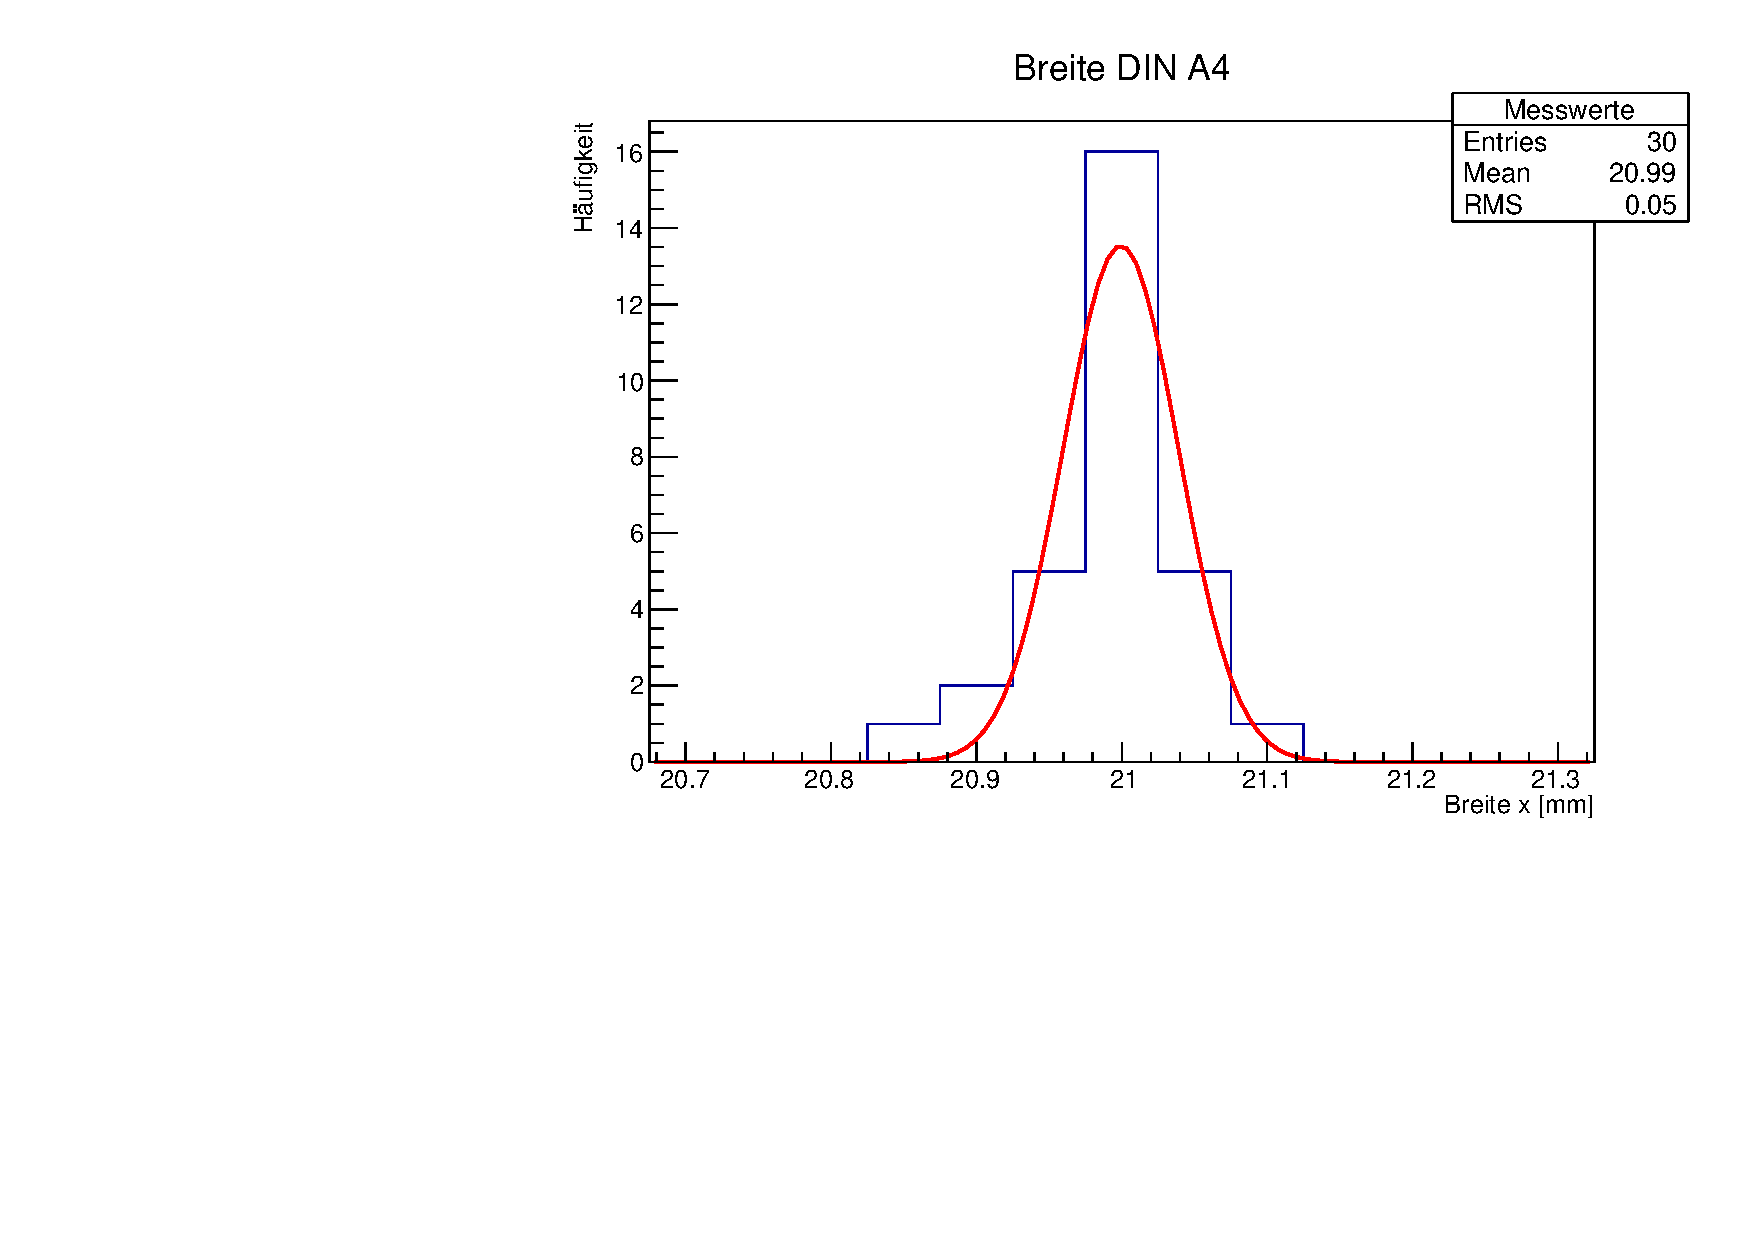
\includegraphics[width=1.00\textwidth]{00_einl/messung_histo.pdf}
	\captionof{figure}{Häufigkeitsverteilung der Messwerte aus Tabelle \ref{tab:MessungDINA4}}
	\label{fig:messung_histo}
\end{minipage}

Die Breite der Häufigkeitsverteilung wird durch die Standardabweichung $\sigma$ beschrieben, je größer diese ist, desto breiter ist die Kurve. Der Wendepunkt der Kurve befindet sich im Abstand $\sigma$ vom Mittelwert. Berechnet man die Fläche unter der Kurve zwischen den beiden Wendepunkten, so ergibt sich:
\begin{equation}
	\frac{1}{\sqrt{2\pi}\sigma}\int_{\bar{x}-\sigma}^{\bar{x}+\sigma}{e^{-\frac{\left(x-\bar{x}\right)^2}{2\sigma^2}}dx} = 0,683
\end{equation}

Das bedeutet, dass die Wahrscheinlichkeit, einen Messwert im Intervall $\left[\bar{x}-\sigma; \bar{x}+\sigma\right]$ zu finden (für $n\rightarrow\infty$), 68,3\% beträgt.

\noindent
Andere oft genutzte Intervalle sind:
\begin{align*}
	\mathrm{1-fache Standardabweichung} &\quad \phantom{0}\bar{x}-\sigma \; \mathrm{bis}\; \bar{x}+\sigma & (68,3\%)\\
	\mathrm{2-fache Standardabweichung} &\quad \bar{x}-2\sigma\; \mathrm{bis}\; \bar{x}+2\sigma & (95,5\%)\\
	\mathrm{3-fache Standardabweichung} &\quad \bar{x}-3\sigma\; \mathrm{bis}\; \bar{x}+3\sigma & (99,7\%)
\end{align*}
%**********************************************************************************************************************
\subsection{Die Unsicherheit eines Messergebnisses}

Da wir als Messergebnis den Mittelwert angeben, ist die Messunsicherheit definiert durch die Frage: \textit{Wie weit weicht der Mittelwert $\bar{x}$ aller Messungen vom wahren Wert $\mu$ ab?}

Diese Abweichung nimmt mit zunehmender Anzahl an Messungen immer weiter ab, der Mittelwert nähert sich dem wahren Wert immer mehr an. Bei einer großen Anzahl an Messungen gilt für die \textit{statistische Unsicherheit des Mittelwertes}:
\begin{important}
	\begin{equation}
		\Delta{\bar{x}} = \frac{\sigma_x}{\sqrt{n}}
	\end{equation}
\end{important}

Den Intervall $\left[\bar{x}-\Delta\bar{x}; \bar{x}+\Delta\bar{x}\right]$ nennt man den \textit{Konfidenzbereich auf dem Vertrauensniveau 68,3\%}. Die Aussage ''Der Messwert beträgt $\bar{x}\pm\Delta\bar{x}$'' bedeutet, dass wenn man den Messvorgang wiederholen würde (mit der gleichen Anzahl an Einzelmessungen $n$), für mindestens $68,3\%$ der auf Grundlage der Messdaten berechneten Konfidenzintervalle der wahre Wert im jeweiligen Konfidenzintervall liegt.

\paragraph{Bemerkung:} Korrektur für kleine Anzahl von Messungen

\begin{table}[t]	
	\centering
		\begin{tabular}[t]{|c|c|c|c|} 
			 & 68,3\% & 95\% & 99,7\% \\ 
			n & t & t & t \\\hline
			2 & 1,84 & 12,71 & 235,8 \\
			3 & 1,32 & 4,30 & 19,21 \\
			4 & 1,20 & 3,18 & 9,22 \\
			5 & 1,15 & 2,78 & 6,62 \\
			6 & 1,11 & 2,57 & 5,51 \\
			8 & 1,08 & 2,37 & 4,53 \\
			10 & 1,06 & 2,26 & 4,09 \\
			20 & 1,03 & 2,09 & 3,45 \\
			30 & 1,02 & 2,05 & 3,28 \\
			50 & 1,01 & 2,01 & 3,16 \\
			100 & 1,00 & 1,98 & 3,08 \\
			200 & 1,00 & 1,97 & 3,04 
		\end{tabular}
	\captionof{table}{Werte der Student-t-Verteilung für verschiedene Konfidenzintervalle}
	\label{tab:Student-t}
\end{table}

\noindent
Liegen nur wenige Messungen vor, so ist die Annahme nicht mehr wahr, dass die Verteilung der Messwerte durch die Normalverteilung beschrieben wird. Stattdessen muss die Student-t-Verteilung verwendet werden. Den Unterschied der beiden Verteilungen berücksichtigen wir durch einen Korrekturfaktor $t$, der Tabelle \ref{tab:Student-t} entnommen werden kann.

\noindent
Für die Unsicherheit des Messwertes gilt dann:
\begin{equation}
 \Delta \bar{x} = \frac{t}{\sqrt{n}}\sigma_x = t\cdot \sigma_{\bar{x}}
\end{equation}

Wie man sieht, geht der Korrekturfaktor für $n\rightarrow\infty$ gegen $t=1$, denn für große Anzahlen an Einzelmessungen nähert sich die Student-t-Verteilung der Normalverteilung an.

%**********************************************************************************************************************
\subsection{Der gewichtete Mittelwert und seine Unsicherheit}

Bei der Bildung des arithmetischen Mittelwertes geht man implizit davon aus, dass alle Messwerte, die in die Mittelung aufgenommen werden, dieselbe Unsicherheit haben. Dies muss nicht immer der Fall sein.\\

Beispiel: \textit{Aus irgendeinem Grund verwenden Sie zur Messung derselben Länge unterschiedliche Massstäbe. Z. Bsp. benutzen Sie für einige Messungen ein Lineal mit einer Genauigkeit von 1~mm, für andere Messungen eine Schieblehre, die eine Auflösung von 0,1~mm hat.}\\

Um diese unterschiedlich genauen Messungen sinnvoll in einem Mittelwert zu kombinieren, benutzt man den \textit{gewichteten Mittelwert}:
\begin{important}
	\begin{equation}
		\bar{x} = \frac{\sum_{i=1}^n{w_i\cdot x_i}}{\sum_{i=1}^n{w_i}}
	\end{equation}
\end{important}
wobei die Wichtungsfaktoren $w_i$ die Kehrwerte der Abweichungsquadrate sind:
\begin{equation*}
	w_i = \frac{1}{\Delta x_i^2}
\end{equation*}
Auf diese Weise tragen Messwerte mit größerer Unsicherheit weniger stark zum Mittelwert bei. Die Unsicherheit des gewichteten Mittelwertes beträgt:
\begin{equation}
	\Delta\bar{x} = \frac{1}{\sum_{i=1}^n{w_i}}
\end{equation}
Sind alle Wichtungsfaktoren $w_i$ gleich, geht der gewichtete Mittelwert in den 'normalen` über, und dessen Abweichung sinkt wieder mit der Wurzel der Zahl der Werte.\\

Der gewichtete Mittelwert gilt strenggenommen nur für normalverteilte Größen. Er wird aber mangels Alternativen auch auf andere statistische oder systematische Abweichungen angewandt. Vor einer Anwendung ist aber zu prüfen, ob die unterschiedlichen Messungen mit dem zugehörigen Konfidenzbereich überlappen. Falls dies nicht der Fall ist, liegt eine zusätzliche, nicht erkannte Abweichung vor (z.B. grobe Fehler).\\

Beispiel:
\textit{Drei Praktikumsgruppen erhalten die Aufgabe, den Durchmesser einer Dose zu bestimmen. Die erste Gruppe erhält eine Schieblehre als Hilfsmittel, die zweite ein 30~cm langes Lineal mit Millimeterskala und die Studierenden der dritten Gruppe müssen mit bloßem Auge den Durchmesser abschätzen:}

\begin{tabular}{|l|l|l|l|} \hline
		& Gruppe 1: & Gruppe 2: & Gruppe 3:\\
		& Durchmesser [mm] & Durchmesser [mm] & Durchmesser [cm]\\ \hline
	Messung 1 & 100,3 & 102,5 & 8 \\
	Messung 2 & 100,2 & 105,0 & 9\\
	Messung 3 & 100,4 & 102,0 & 10 \\
	Messung 4 & 100,1 & 107,0 & 13 \\
	Messung 5 & 100,2 & 100,5 & 6 \\
	Messung 6 & 100,3 & 101,0 & 12 \\
	Messung 7 & 100,5 & 102,5 & 9\\
	Messung 8 & 100,0 & 103,0 & 11\\
	Messung 9 & 100,4 & 102,5 & 12\\
	Messung 10 & 100,3 & 103,5 & 8 \\ \hline
	Mittelwert & 100,270 & 102,95 & 9,8\\ \hline
	Std. abw. & 0,047 & 0,60 & 0,70\\ \hline
\end{tabular}

\textit{Der Mittelwert aus allen diesen Messungen für den Dosendurchmesser $d$ ergibt:}
\begin{align}
	\bar{d} & = \frac{\frac{100,27}{0,047^2}+\frac{102,95}{0,60^2}+\frac{98}{7^2}}{\frac{1}{0,047^2}+\frac{1}{0,60^2}+\frac{1}{7^2}}\;\mathrm{mm} = 100,286\;\mathrm{mm}\\
	\Delta\bar{d} & = \frac{1}{\sqrt{\frac{1}{0,047^2}+\frac{1}{0,60^2}+\frac{1}{7^2}}}\;\mathrm{mm} = 0,047\;\mathrm{mm}
\end{align}
\textit{Als Messwert für den Durchmesser ergibt sich also: $d = (100,286\pm 0,047)\;\mathrm{mm}$.}
%**************************************************************
% Hier noch was zu Geräten und Aufspüren systematischer Fehler?
%**************************************************************

%**********************************************************************************************************************
%**********************************************************************************************************************
\section{Indirekte Messung: Fehlerfortpflanzung}

Wenn sich die gesuchte Größe aus zwei oder mehr einzeln gemessenen Größen zusammensetzt, so nennt man die Bestimmung der zusammengesetzten Größe eine \textit{indirekte Messung}. Ein Beispiel dafür ist schon die einfache Bestimmung der Fläche eines DIN A4 Blattes, die wir uns früher schon angeschaut haben.

Wie wir wissen, sind die einzelnen, direkten Messungen mit Unsicherheiten behaftet. Wie können wir aus diesen die Ungenauigkeit der indirekten Messung der zusammengesetzten Größe berechnen?

%**********************************************************************************************************************
\subsection{Größtfehlerbetrachtung}

Die einfachste Möglichkeit, den Fehler abzuschätzen, ist die Annahme, dass die Unsicherheiten aller Einzelgrößen voll zur Gesamtunsicherheit beitragen und sich nicht untereinander beeinflussen (man sagt \textit{sie sind nicht korreliert}).

Rechnerisch wird das umgesetzt, indem man in die Formel zur Berechnung der gesuchten zusammengesetzten Größe die Einzelmessungen $x_i \pm \Delta x_i$ so einsetzt, dass das Ergebniss maximal wird. Anschliessend wird der Vorgang so wiederholt, dass das Ergebnis minimal wird. Die Differenz der beiden Ergebnisse bezeichnet man als den \textit{Größtfehler}.\\

%\noindent
Dieses Verfahren berücksichtigt den statistischen Zusammenhang der einzelnen Beiträge nicht, daher liefert es im Allgemeinen zu große Werte für die Unsicherheit. Darüber hinaus können sich rechnerische Schwierigkeiten ergeben, wenn z. Bsp. die entsprechende Größe in einer Summe im Nenner und im Zähler der Formel vorkommt. In diesem Fall ist es schwierig herauszufinden, ob die positive oder die negative Abweichung den größten bzw. den kleinsten Wert ergibt. Dieses Verfahren ist daher nur für den Notfall geeignet, liefert jedoch oft eine brauchbare Abschätzung.

%**********************************************************************************************************************
\subsection{Gauß'sche Fehlerfortpflanzung}

Betrachten wir eine Größe $g$, die nicht direkt gemessen werden kann, sich aber aus mehreren direkt gemessenen Größen $x$, $y$, $z$,... berechnen läßt:
\begin{equation}
	g = g(x,y,z,...)
\end{equation}
Der Einfachheit halber wollen wir uns im Folgenden auf die drei Messgrößen $x$, $y$ und $z$ beschränken, die Rechnungen können jedoch prinzipiell mit beliebig vielen Messgrößen durchgeführt werden.

Wir gehen davon aus, dass die Messserien für die Größen $x$, $y$ und $z$ normalverteilt sind. Dann kann der Mittelwert $\bar{g}$ der gesuchten Größe bestimmt werden, indem man die Mittelwerte der Messgrößen in die Formel einsetzt:
\begin{important}
	\begin{equation}
		\bar{g} = g(\bar{x},\bar{y},\bar{z})
	\end{equation}
\end{important}

Wenn die Messgrößen $x$, $y$ und $z$ statistisch unabhängig voneinander sind, man sagt \textit{unkorreliert}, dann kann die gesamte Unsicherheit wie folgt berechnet werden:
\begin{important}
	\begin{equation}
		\Delta\bar{g} = \sqrt{\Delta\bar{x}^2 \cdot \left(\frac{\partial g}{\partial x} \right)^2_{\bar{x},\bar{y},\bar{z}} + \Delta\bar{y}^2 \cdot \left(\frac{\partial g}{\partial y} \right)^2_{\bar{x},\bar{y},\bar{z}} + \Delta\bar{z}^2 \cdot \left(\frac{\partial g}{\partial z} \right)^2_{\bar{x},\bar{y},\bar{z}}}
	\end{equation}
\end{important}

Diese Formel ist bekannt als die \textit{Gauß'sche Fehlerfortpflanzung}, wenn für die Unsicherheiten $\Delta\bar{x}$, $\Delta\bar{y}$, $\Delta\bar{z}$ die jeweilige Standardabweichung eingesetzt wird.

Die Ausdrück $\partial g/\partial x$, $\partial g/\partial y$ und $\partial g/\partial z$ stehen dabei für die partiellen Ableitungen der Formel zur Berechnung von $g$ nach den Variablen $x$, $y$ und $z$.

\paragraph{Beispiel:} Messung der Dichte eines Quaders\\
\textit{
Die Dichte eines Quaders ergibt sich aus seiner Masse $m$ und seinem Volumen $V = x\cdot y\cdot z$, wenn $x$, $y$ und $z$ die Kantenlängen sind, nach der Formel
\begin{equation}
	\rho = \frac{m}{V} = \frac{m}{x\cdot y\cdot z}
	\label{eq:Dichte}
\end{equation}
Bei der Messung der Masse und der Kantenlängen findet man die Werte $\bar{m}\pm \sigma_m$, $\bar{x}\pm \sigma_x$, $\bar{y}\pm \sigma_y$ und $\bar{z}\pm \sigma_z$. Die partielle Ableitung von Gleichung \ref{eq:Dichte} nach der Masse $m$ ist:
\begin{equation*}
	\frac{\partial \rho}{\partial m} = \frac{1}{x\cdot y\cdot z}
\end{equation*}
Die partielle Ableitung nach $x$ lautet (für die anderen beiden Richtungen genauso vorgehen):
\begin{equation*}
	\frac{\partial \rho}{\partial x} = -\frac{1}{x}\cdot\frac{m}{x\cdot y\cdot z}
\end{equation*}
Damit ergibt sich für die Unsicherheit der Dichte:
\begin{equation}
	\Delta\bar{\rho} = \sqrt{\Delta\bar{x}^2\left(-\frac{1}{\bar{x}}\frac{m}{\bar{x}\bar{y}\bar{z}} \right)^2 + \Delta\bar{y}^2\left(-\frac{1}{\bar{y}}\frac{m}{\bar{x}\bar{y}\bar{z}} \right)^2 + \Delta\bar{z}^2\left(-\frac{1}{\bar{z}}\frac{m}{\bar{x}\bar{y}\bar{z}} \right)^2 + \Delta\bar{m}^2\left(\frac{1}{\bar{x}\bar{y}\bar{z}}\right)^2}
\end{equation}
In diese Gleichung sind jetzt nur noch die jeweiligen Mittelwerte und Unsicherheiten einzusetzen, um die Unsicherheit der Dichte zu berechnen.
}\\

Falls die einzelnen Messgrößen nicht normalverteilt sind, oder wenn sie nicht statistisch von einander unabhängig sind, muss man bei der Fortpflanzung der Unsicherheiten noch einen Korrekturfaktor berücksichtigen, der diese Korrelation der Messgrößen beschreibt. Diesen nennt man den \textit{Korrelationskoeffizienten}.

%**********************************************************************************************************************
\subsection{Fortpflanzung systematischer Abweichungen}

Systematische Abweichungen entziehen sich naturgemäß einer statistischen Behandlung. Man kann insbesondere nicht davon ausgehen, dass es unwahrscheinlich ist,
dass alle Abweichungen der Beteiligten Einzelgrößen gleichzeitig extremal sind.\\

Beispiel:
\textit{Eine Veränderung der Umgebungstemperatur bei der Messung zieht eine Abweichung aller Längenmessungen gemeinsam nach sich, da der Maßstab natürlich bei jeder Messung
'falsch' ist. Man muss also in diesem Fall davon ausgehen, dass die Abweichungen nicht quadratisch addiert werden dürfen, sondern linear addiert werden müssen. Der Einfluss jeder
Einzelabweichung muss voll auf die Gesamtabweichung durchschlagen.}\\

\textit{Im Fall einer systematischen Abweichung der Längenmessung durch einen nicht gleichmäßig geteilten Maßstab erscheint es jedoch sinnvoll anzunehmen, dass je nach Position die Abweichung unterschiedlich ist. Entsprechend kann man auch davon ausgehen, dass nicht gerade alle Abweichungen zum gleichen Zeitpunkt in die gleiche Richtung gehen. Hier ist also eine quadratische Addition sinnvoll.}\\

Es hängt also vom Einzelfall ab welche Methode der Fortpflanzung bei einer systematischen Abweichung angewandt werden muss. Die lineare Addition bei potentiell statistisch gekoppelten Vorgängen oder die quadratische Addition bei definitiv statistisch unabhängigen Vorgängen.\\
Sei beispielsweise die Größe $g$ aus drei Variablen $x, y, z$ zusammengesetzt, die jeweils die systematischen Unsicherheiten $\Delta x, \Delta y, \Delta z$ haben. Dann erfolgen lineare und quadratische Addition wie folgt:

\textbf{Lineare Addition}
\begin{equation} \label{eq:error_lin_add}
	\Delta\bar{g} = \left|\Delta\bar{x}\cdot \left[\frac{\partial g}{\partial x}\right]_{\bar{x}, \bar{y}, \bar{z}}\right|
								+ \left|\Delta\bar{y}\cdot \left[\frac{\partial g}{\partial y}\right]_{\bar{x}, \bar{y}, \bar{z}}\right|
								+ \left|\Delta\bar{z}\cdot \left[\frac{\partial g}{\partial z}\right]_{\bar{x}, \bar{y}, \bar{z}}\right|
\end{equation}

\textbf{Quadratische Addition}
\begin{equation} \label{eq:error_quad_add}
	\Delta\bar{g} = \sqrt{\Delta\bar{x}^2\cdot \left[\frac{\partial g}{\partial x}\right]^2_{\bar{x}, \bar{y}, \bar{z}}
											+ \Delta\bar{y}^2\cdot \left[\frac{\partial g}{\partial y}\right]^2_{\bar{x}, \bar{y}, \bar{z}}
											+ \Delta\bar{z}^2\cdot \left[\frac{\partial g}{\partial z}\right]^2_{\bar{x}, \bar{y}, \bar{z}}}
\end{equation}
%**********************************************************************************************************************
\subsection{Verkn"upfung statistischer und systematischer Unsicherheiten}

Auch bei der Verkn"upfung systematischer und statistischer Unsicherheiten ist die Frage nach de Kopplung der Gr"o{\ss}en zu beachten. Die Frage, ob die statistische Unsicherheit von der systematischen Abweichung abh"angig ist oder nicht, ist jedoch letztlich nicht beantwortbar. Entsprechend werden in der Literatur auch beide Meinungen vertreten.\\

\noindent
\textbf{Im Praktikum} wollen wir vom konservativen Fall ausgehen und annehmen, dass die beiden Beitr"age nicht voneinander unabh"angig sind und befolgen die folgenden Schritte:
\begin{enumerate}
	\item Bestimmung der statistischen Unsicherheit aus allen Einzelgr"o{\ss}en mittels \textit{quadratischer Addition} nach Gleichung \ref{eq:error_quad_add}.
	\item Bestimmung der systematischen Unsicherheit aus \textit{linearer Addition} aller Einzelgr"o{\ss}en nach Gleichung \ref{eq:error_lin_add}.
	\item Verkn"upfung der statistischen und systematischen Unsicherheit mittels normaler linearer Addition, nicht Gleichung \ref{eq:error_lin_add}, zur Gesamtunsicherheit, welche dann beim Ergebnis angegeben wird.
\end{enumerate}
%**********************************************************************************************************************
\begin{todo}
	Einen Abschnitt über systematische Unsicherheiten und wie man sie abschätzt.
\end{todo}

%**********************************************************************************************************************
%**********************************************************************************************************************
\section{Graphische Auswertung bei korrelierten Messwerten}

Dein einfachste Beziehung zwischen zwei Messgrößen ist die \textit{lineare Abhängigkeit}
\begin{equation}
	y(x) = a\cdot x + b
\end{equation}
mit den beiden freien Parametern $a$ und $b$.